% This is samplepaper.tex, a sample chapter demonstrating the
% LLNCS macro package for Springer Computer Science proceedings;
% Version 2.20 of 2017/10/04
%
\documentclass[runningheads]{llncs}
%
\usepackage{graphicx}
\usepackage[acronym]{glossaries}
\usepackage{mathtools}
\usepackage{amssymb}
\usepackage{float}
\graphicspath{ {./images/} }
\newacronym{ann}{ANN}{Artificial Neural Network}
\newacronym{mse}{MSE}{Mean Squared Error}
\newacronym{mae}{MAE}{Mean Absolute Error}
\newacronym{anns}{ANNs}{Artificial Neural Networks}
\newacronym{cnns}{CNNs}{Convolutional Neural Networks}
\newacronym{rnns}{RNNs}{Recurrent Neural Networks}
\newacronym{bptt}{BPTT}{Back Propagation Through Time}
\newacronym{vae}{VAE}{Variational Autoencoders}
\newacronym{drl}{DRL}{Deep Reinforcement Learning}
\usepackage[hyphens]{url}
\usepackage[hidelinks]{hyperref}
\hypersetup{breaklinks=true}
% Used for displaying a sample figure. If possible, figure files should
% be included in EPS format.
%
% If you use the hyperref package, please uncomment the following line
% to display URLs in blue roman font according to Springer's eBook style:
% \renewcommand\UrlFont{\color{blue}\rmfamily}

\begin{document}
%
\title{Neural Networks and Deep Learning }
%
%\titlerunning{Abbreviated paper title}
% If the paper title is too long for the running head, you can set
% an abbreviated paper title here
%
\author{Mohamed Hesham Ibrahim Abdalla \and
Slim Abdennadher \and
Alia Elbolock}
%
\authorrunning{M. Abdalla et al.}
% First names are abbreviated in the running head.
% If there are more than two authors, 'et al.' is used.
%
\institute{German University in Cairo, Cairo, Egypt}
%  \and
% Springer Heidelberg, Tiergartenstr. 17, 69121 Heidelberg, Germany
% \email{lncs@springer.com}\\
% \url{http://www.springer.com/gp/computer-science/lncs} \and
% ABC Institute, Rupert-Karls-University Heidelberg, Heidelberg, Germany\\
% \email{\{abc,lncs\}@uni-heidelberg.de}}
%
\maketitle              % typeset the header of the contribution
%
\begin{abstract}
The abstract should briefly summarize the contents of the paper in
15--250 words.

\keywords{Neural Networks  \and Deep Learning \and Machine Learning}
\end{abstract}
%
%
%
\section{Introduction}

\gls{anns} and perceptrons are intelligent units that have taken inspiration
from biology, especially the brain \cite{hassoun1995fundamentals}. \gls{anns} work by taking labeled inputs
and then trying to find a mathematical rule or function that could answer the question
of which label belongs to which input, and later identify labels of new inputs that have never been seen before by the network. For example, inputs could be human faces (as images) and the labels are 
a binary value for the gender of that face.

The history of \gls{anns} and perceptrons goes back to the 50's and the 60's when 
the first known perceptrons was created. In 1958 Frank Rosenblatt began working on the perceptrons.  
This perceptrons was build completely on hardware and the idea behind it is very similar 
to modern neurons or perceptrons (Figure \ref{fpp}). It was used to classify continuous inputs by 
by applying a weighted sum of the inpus and subtracting a bias (constant value) and 
then the output is given as a number from two possible values (0 or 1).
\begin{figure}[H]
    \label{fpp}
    \centering
    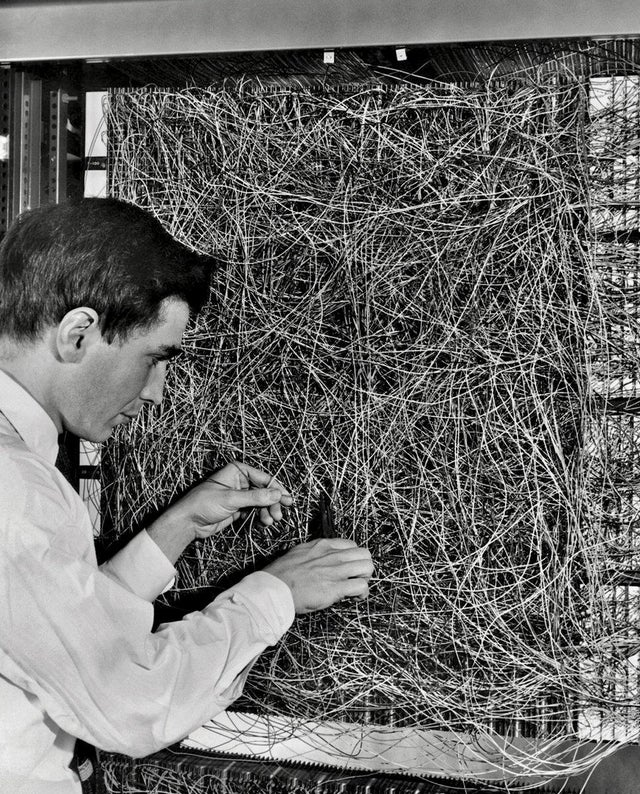
\includegraphics[height=4cm]{imge1}
    \caption{Frank Rosenblatt with a Mark I Perceptron computer \cite{frankpic}.}
\end{figure}
Shortly after the first perceptrons, 
the research on \gls{anns} stopped until 1981, due to fear and unfulfilling results.
After this peroid, many institutions and researchrs began working on \gls{anns} again, such as 
US-Japan Joint Conference on Cooperative/ Competitive Neural Networks \cite{amari1982competition}, Schmidhuber \& Hochreiter \cite{hochreiter1997long} and Yann LeCun \cite{lecun1998gradient}. 



\section{Mathematical Background and Concept}
\gls{anns} learn how to accomplish a task by excuting two main steps:
forward propagation and back propagation. Forward propagation is the process of
predicting labels and computing how deviated these labels from the ones provided in the input data.
On the other hand, back propagation tries to correct the predictions by minimizing
the diffrence between the input labels and the predicted labels. 
\subsection{Forward Propagation}
\label{fb}
\gls{anns} consist of layers where each layer has neurons which are connected via links (Figure \ref{nn}). Each neuron gets inputs and produces an output. 
Each input is given a certain weight which makes that specific input has more or less effect on the output of the neuron.

\begin{figure}[H]
    \label{nn}
    \centering
    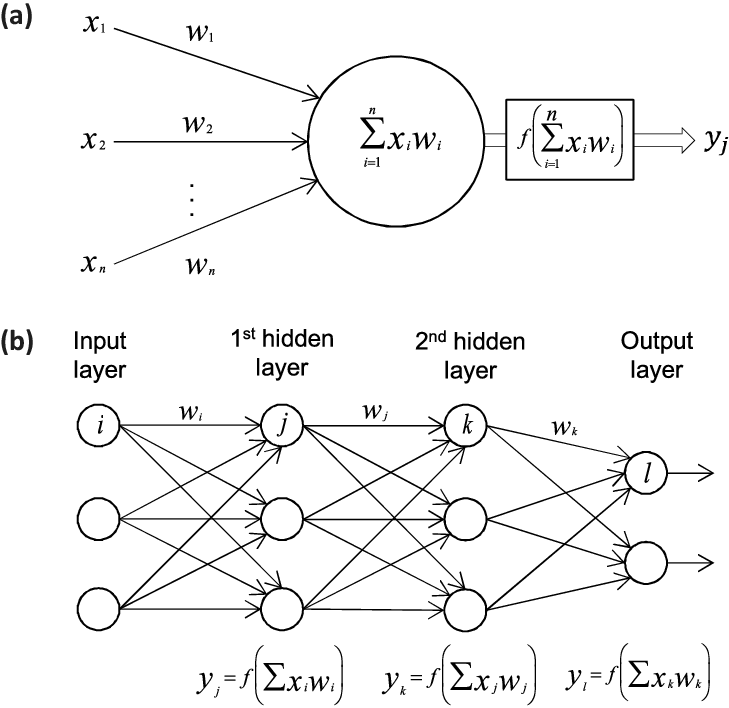
\includegraphics[height=8cm]{nn}
    \caption{(a) A single-layer \gls{ann} where the first layer has only one neuron. 
    (b) A multi-layer \gls{ann} with 2 hidden layers \cite{nnimage}. }
\end{figure}

Neurons calculate their output by multiplying their inputs by their weights and applying a bias to the multiplication. Eqaution \ref{z}
shows a linear mapping of a single input.
\begin{equation}
\label{z}
    z^i = W^Tx^i + b
\end{equation}
where $z^i$ is the linear mapping of the $i$th example,  $W$ $\in$ $ R^{1 \times n_{x}} $ is the weight vector of the form $[w_1, w_2, ... w_{n_{x}}]$, 
$x^i$ $\in$ $ R^{n_{x}\times1} $ is the input vector of the form $[x_1, x_2, ... x_{n_{x}}]$ of the $i$th example and $n_{x}$ is the number
of features of the input vector (input size).

\begin{figure}[H]
    \label{exsep}
    \centering
    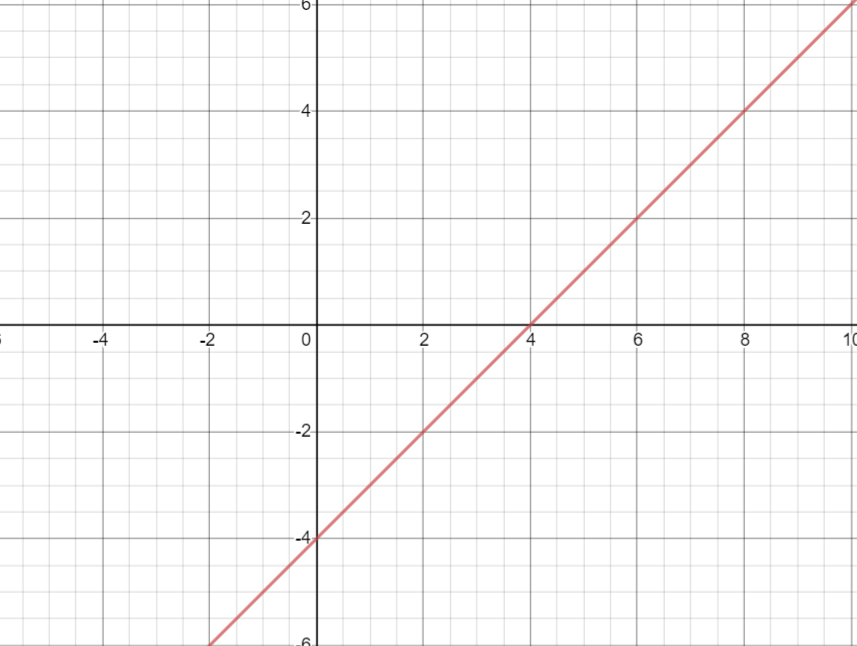
\includegraphics[height=4cm]{sepfig}
    \caption{A Figure that shows a sepration line with $n_{x}$ = 1, $W$ = 1, $b$ = -4
    ($1x-4$).}
\end{figure}

This mapping is then forwaded to an activation function (Eqaution \ref{a}).
Activation functions are used to limit the linear transformation output.
\begin{equation}
    \label{a}
        a^i = g(z^i)
\end{equation}
where $a^i$ is the output of the activation function (unit activation) on the linear mapping of the $i$th example.

To avoid manaully looping over each example and summing the output, all of the variables are used
as vectors.

\begin{equation}
    \label{zeq1}
        Z^{[l]} = W^{T[l]}A^{[l-1]} + b^{[l]}
\end{equation}

\begin{equation}
    \label{zeq2}
        A^{[l]} = g^{[l]}(Z^{[l]})
\end{equation}

where $Z^{[l]}$ is the linear mapping of the $l$th layer, $W^{T[l]} \in R^{n^{[l]} \times n^{[l-1]}}$ is the weight vector of the 
$l$th layer, $b^{[l]} \in R^{n^{[l]}}$ is the bias vector of the $l$th layer, $A^{[l-1]}$ is the activation unit
of the previous layer ($A^{[0]}$ = $X$), $A^{[l]}$ is the activation unit of the $l$th layer, 
$g()^{[l]}$ is the activation function of the $l$th layer, $n^{[l]}$ number of units (neurons) in the $l$ layer
and $n^{[l-1]}$ is the number of units in the previous layer ($l - 1$)th layer.


The choice of the activation function vary depending on the given data (inputs). 
In general, 
there are three main categories of the activation function: binary, linear and non-linear. 
Binary or threshold functions output a binary value depending on the input. 
For example, the step function outputs +1 in case $z^i$ is greater than or eqaul to 0 and -1 otherwise (Eqaution \ref{b}).
Binary functions can not deal with categorical data, therefore they are not widely used.
\begin{equation}
    \label{b}
f(x) = \left\{ \begin{array}{ll} +1 \quad z^i \leq 0 \\ -1 \quad \text{otherwise} \end{array} \right.
\end{equation}

Another type of activation functions is linear. 
Linear functions forward the input directly to the output without any transformation.
This is useful in problems where the output is continuous. For example, predicting house prices.

Although all of the previous functions are useful for some sitautions, 
they fail to find a pattern if the data is non-linearly separable, 
since the function will only be able to draw a linear decesion boundary that can only devide the data into two groups.
Therefore, other functions are used to find non-linear sepration between the data. 
(Figure \ref{actfig}) shows some widely used non-linear activation functions.

\begin{figure}[H]
    \label{nls}
    \centering
    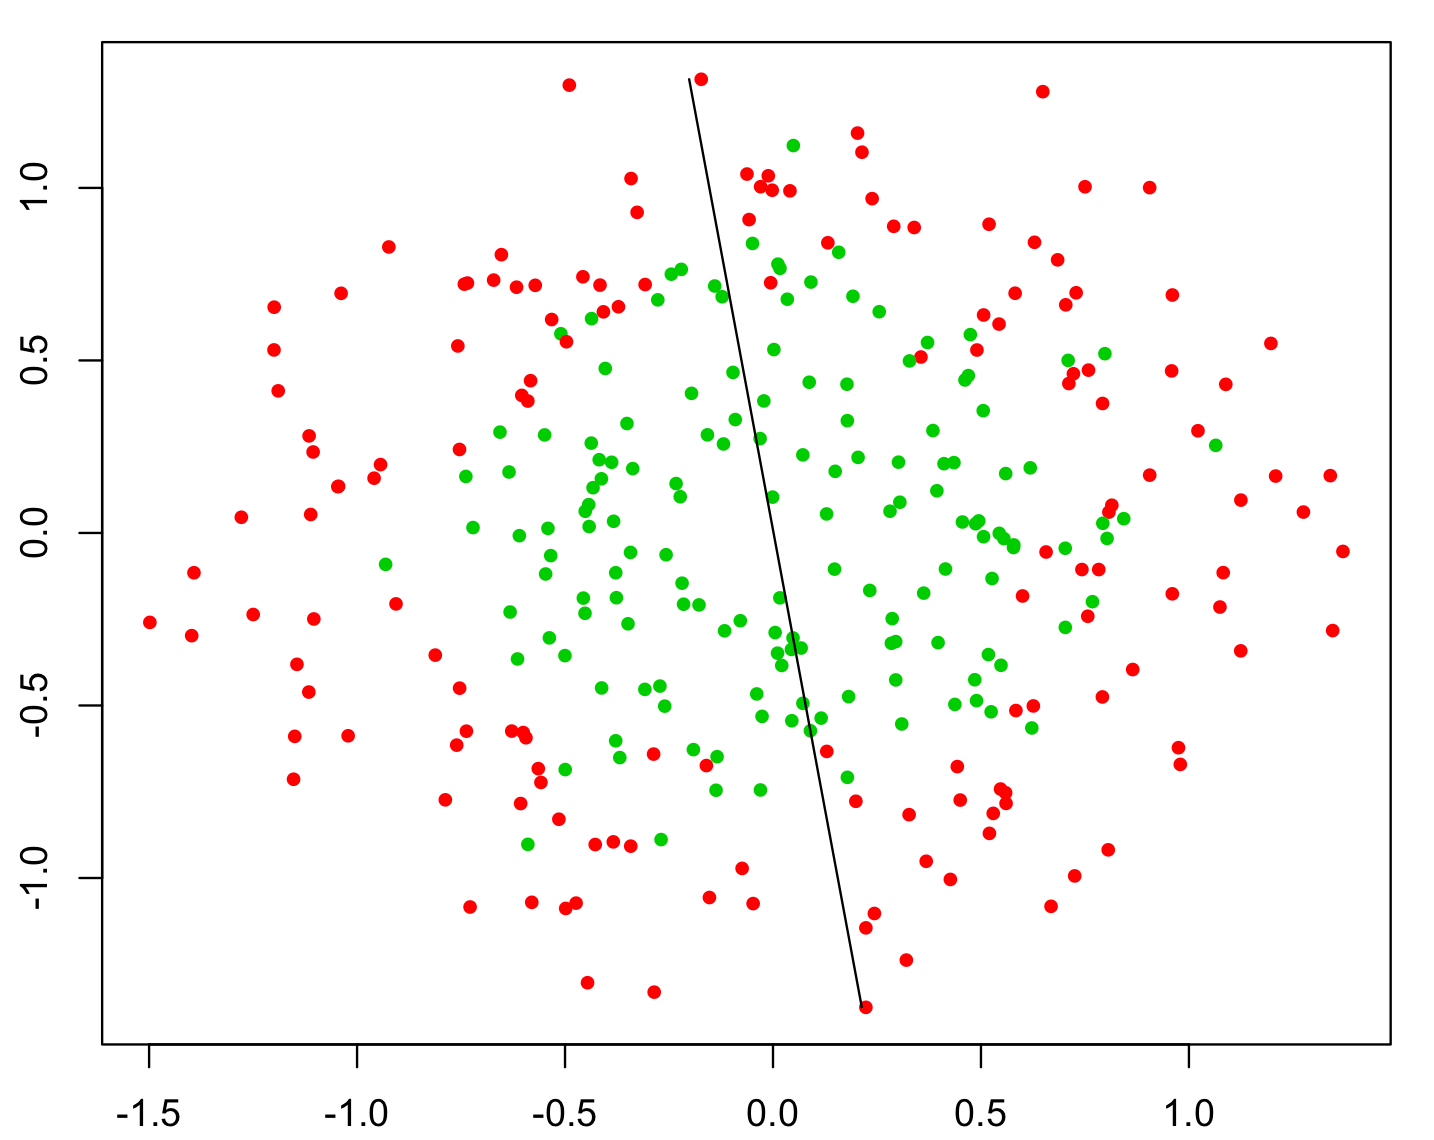
\includegraphics[height=5cm]{linear}
    \caption{Example of a linear activation function on non-linearly separable data \cite{nonsep}. }
\end{figure}

After calculating the activation unit for the inputs, 
a loss function $L$ is calculated for each prediction to measure 
how different the prediction is from the real data. the formula of the loss function varies based on the type of the labels.
For example, if the labels are binary values (consisting of two classes), 
Log Loss could be used. 
This loss function pentalize the wrong prediction by applying the negative sign 
to the log, since the log of the values between 0.0 and 1.0 will output negative numbers
(increse the loss for wrong predictions) (Eqaution \ref{log}). 

\begin{equation}
    \label{log}
L_{i} = -y_{i} \log{(\hat{y_{i}})} - (1 - y_{i})\log{(1-\hat{y_{i}})}
\end{equation}
where $L_{i}$ is the loss function of the $i$th example, $y_{i}$ is the label of the $i$th example,
$\hat{y_{i}}$ is the prediction of the $i$th example.


Alternatively, if the labels are continuous, 
\gls{mae} or \gls{mse} are used (Eqaution \ref{maeq} and \ref{mseq}).

\begin{equation}
    \label{maeq}
    MAE_{i} = |y_{i} - \hat{y_{i}}|
\end{equation}
\begin{equation}
    \label{mseq}
    MSE_{i} = {(y_{i} - \hat{y_{i}})}^2
\end{equation}
where $MAE_{i}$ is the \gls{mae} of the $i$th example, $MSE_{i}$ is the \gls{mse} of the $i$th example,  
$y_{i}$ is the label of the $i$th example,
$\hat{y_{i}}$ is the prediction of the $i$th example.


\subsection{Back Propagation}

Back propagation is the process of tunning the input weights of each 
neuron to correctly predict new labels. In other words,
finding the weights that minimize the loss function. These weights are calculated through
an algorithm called gradient descent \cite{lemarechal2012cauchy}. Gradient descent is the process of iteratively updating
the parameters of a function (input weights) in the direction of the steepest descent until a local minima is reached.
To give a better idea, we can imagine the parameter space as a surface from where we follow
the direction of the slope downhill until we reach a valley (Figure \ref{gd}).
Moreover, the slope is calculated by finding the first partial derivative of a function $J$ in respect to every parameter of the function (Eqaution \ref{gdu}). 

\begin{figure}[H]
    \label{gd}
    \centering
    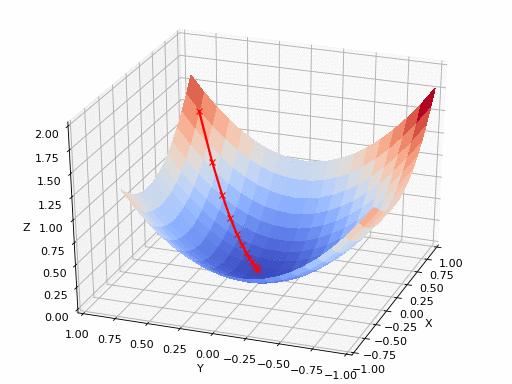
\includegraphics[height=4cm]{gd}
    \caption{Gradient descent visualization where the function is moving from a local maxima to a local minima \cite{gdwiki}.}
\end{figure}

\begin{equation}
    \label{gdu}
w_{i} = w_{i} - \eta \frac{\partial J(W)}{\partial w_{i}}
\end{equation}

where $w_{i}$ is the $i$th parameter, $\eta$ is the learning rate (a parameter used to control how large a step is).

in case of a multi-layer \gls{ann} with $L$ layers, the gradient is instead calculated 
with the chain rule where the partial derivative is applied on each of the hidden layers
till the first layer is reached.

\begin{equation}
    \label{gdu}
w_{i} = w_{i} - \eta (\frac{\partial J(g_{i}(W))}{\partial g_{i}(W)}\frac{\partial g_{i}(W)}{\partial W})
\end{equation}

Since in the multi-layer \gls{anns} the derivative is also applied to the activation functions,
the choice of which activation function to be used is crucial. For example, using 
tanh or sigmoid functions may result in a slower learning process, as the first derivative of these functions
is not so steep on extremely high or extremely low values (Figure \ref{actfig}).

\begin{figure}[H]
    \label{actfig}
    \centering
    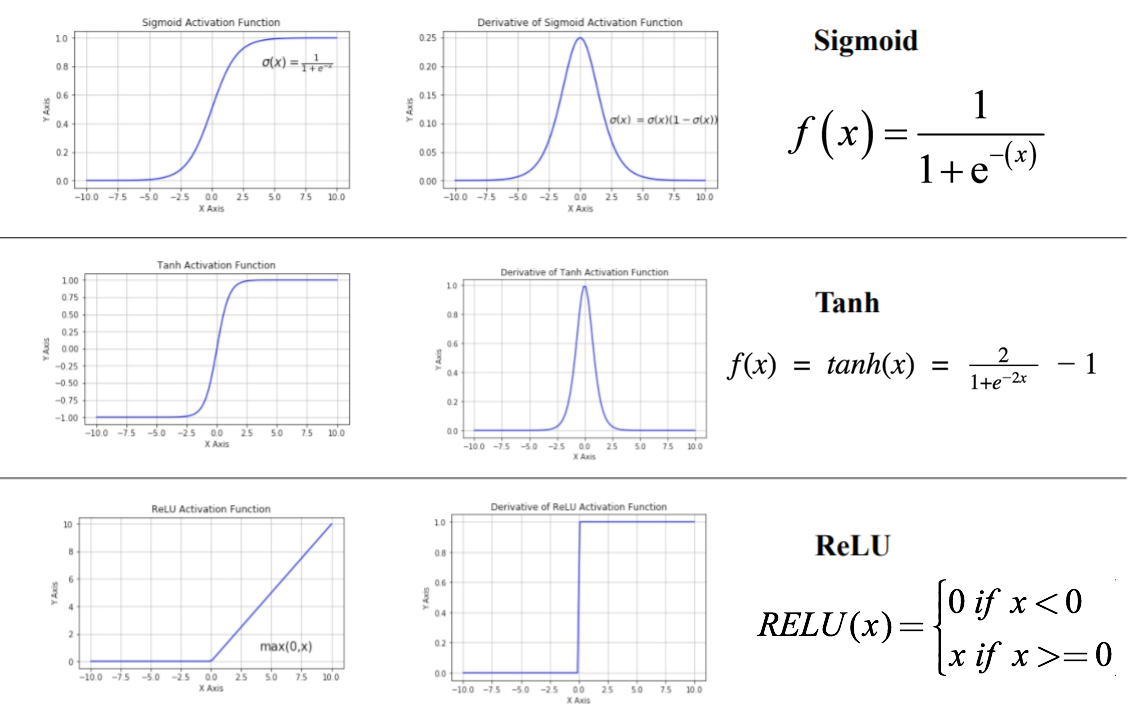
\includegraphics[height=6cm]{actfig}
    \caption{A figure of some activation functions where the first one is sigmoid, the second is Tanh and the last is ReLU \cite{sdc}.}
\end{figure}



\section{Applications and Architectures}

In this section, we are going to discuss some of the architectures of \gls{anns}
and their applications.

\subsection{Convolutional Neural Networks}

While machines can calculate and do other tasks faster than humans,
they can not sense or see objects. Therefore, many researchers
tried to make machines mimic human vision through the field of classical Computer Vision \cite{hoffmann1992computer}.
However, this approach was hard to implement since an explicit algorithm 
has to be written. For example, if we want to do a task like
face detection, we have to define what a face is and how
far the eyes are away from each other and define many other measurements. This is not 
an easy task, because to generalize well, the algorithm has to 
cover every feature a human face can ever have and its measurements. Deep Learning 
and \gls{anns} can solve this problem by just providing enough data
(face images) and applying non-linearity to it.
% \begin{figure}{H}
%     \label{dcnn}
%     \centering
%     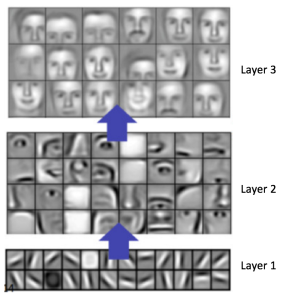
\includegraphics[height=7cm]{dcnn}
%     \caption{a 2x2 Max Pooling operator on a 4x4 gray scale image.
%     \cite{lee2009convolutional}}
% \end{figure}
Images are presented as pixels and each pixel has a certain value.
an \gls{ann} can take the pixels as parameters for the network 
and connect them to the neurons. To take all the pixels from
one image, the \gls{ann} has to provide many parameters. For example,
a gray scale image with 28x28 size will be presented in 784 parameters, 
since the image has to be flatten before being processed by the \gls{ann}.
Therefore, other approaches were used to process images with lower dimensionality.
\gls{cnns} use the “convolution” operator \cite{lecun1998gradient}. The main purpose of that 
operator is to extract only the important features from an image while
still preserving the spatial relationship between its pixels. This is 
done using a sqaure of weights (filter) which
gets multiplied by the image values (index-wise) and then producing an output called a feature map (Figure \ref{fm}).


\begin{figure}[H]
    \label{fm}
    \centering
    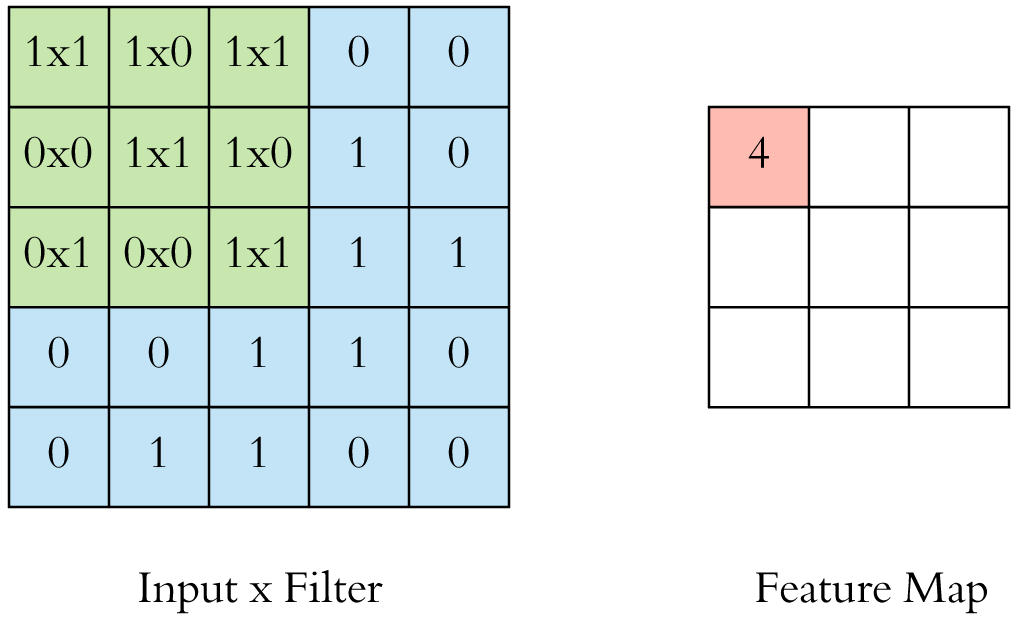
\includegraphics[height=4cm]{filter}
    \caption{A filter of size 3x3 applied on a 5x5 binary image \cite{appf}.}
\end{figure}

% \begin{figure}
%     \label{ff}
%     \centering
%     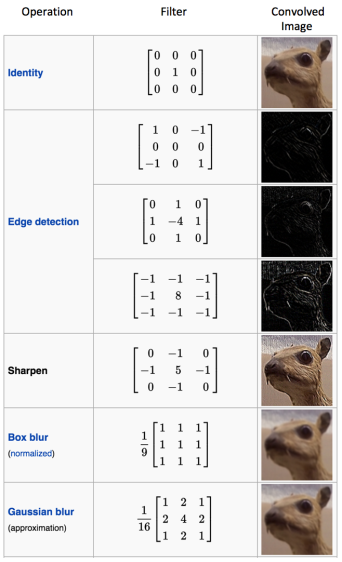
\includegraphics[height=6cm]{filters}
%     \caption{Diffrent filters(?)
%     https://towardsdatascience.com/applied-deep-learning-part-4-convolutional-neural-networks-584bc134c1e2}
% \end{figure}

A non-linear function is then applied to the feature map (Section \ref{fb}).
To further reduce dimensionality, \gls{cnns} uses the spatial pooling operator.
This operator has diffrent types: Max, Average, Sum etc. 
When Max Pooling is used, the largest element is chosen from each window.
Figure \ref{mp} shows a 2x2 Max Pooling operator.


\begin{figure}{H}
    \label{mp}
    \centering
    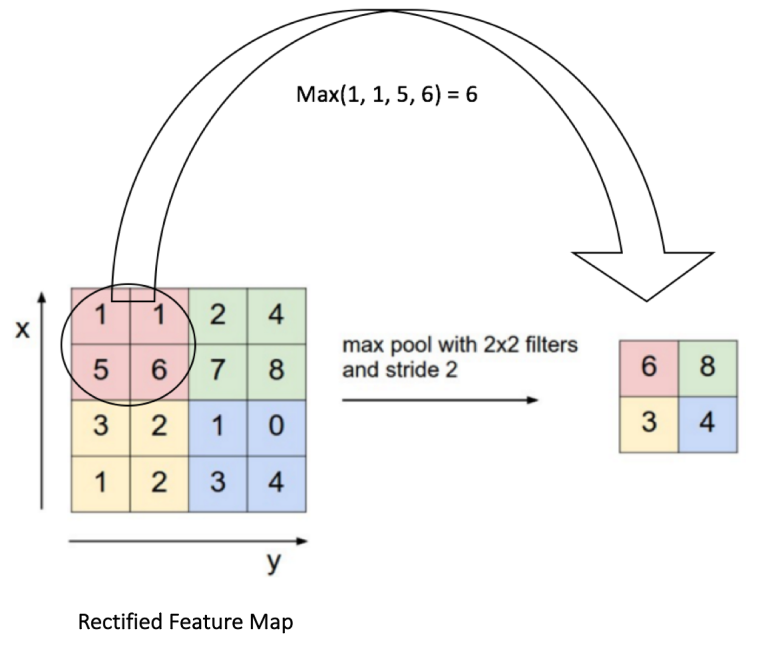
\includegraphics[height=5cm]{max_pool}
    \caption{a 2x2 Max Pooling operator on a 4x4 gray scale image \cite{maxpool}.}
\end{figure}

The learning part in this \gls{ann} is the filter weights. However, we 
still need to define the height and width parameters of the filter on each layer, how
many layers will the \gls{cnns} use and many other parameters. In general, 
the more layers the \gls{ann} has, the more it will be able to detect complex 
relations between pixels (shapes).

After finishing the previous operator, \gls{cnns} are usaully connected with 
a dense \gls{ann} to be able to predict/ classify a certain image. Figure \ref{dcnnp} 
shows an example process of a CNN.

\begin{figure}{H}
    \label{dcnnp}
    \centering
    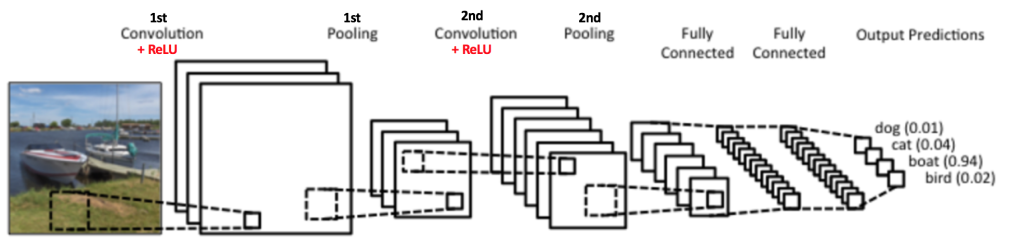
\includegraphics[height=3cm]{dcnnp}
    \caption{A CNN applied on a boat image to detect if it falls in 
    dog, cat, boat or bird categories \cite{cnnpro}.}
\end{figure}

\gls{cnns} have many applications, especially in healthcare. For instance, 
\gls{cnns} outperformed expert radiologists at detection breast cancer \cite{mckinney2020international} (Figure \ref{can}).

\begin{figure}{H}
    \label{can}
    \centering
    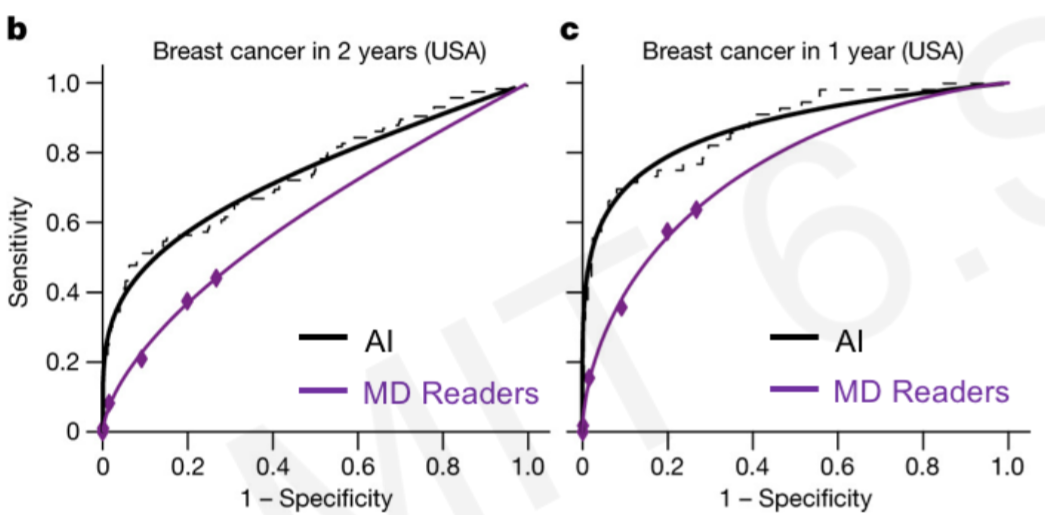
\includegraphics[height=5cm]{cancer}
    \caption{A figure showing that AI and \gls{cnns} can outperform RD Readers \cite{mitlecthree}.}
\end{figure}



\subsection{Recurrent Neural Networks}

\gls{rnns} is an \gls{ann} architecture which is used to predict a step in a sequence \cite{hochreiter1997long}.
For example, consider the sentence "Mathematics is my favorite subject, therefore I want to study \_\_\_ in college".
A valid guess for the blank can be Mathematics or Engineering. Without seeing
what is before the comma, we would not have gussed the word correctly.
normal \gls{anns} architectures (Section \ref{fb}) propagate the inputs in one way and therefore 
the inputs are not aware of each other (parameter sharing) 
(not able to see what is before the comma because it process each word separately).
\gls{rnns} address this problem by having an internal state (also called a hidden state) which gets 
updated every time when a new input is recieved (Eqaution \ref{rnn}). 

\begin{equation}
    \label{rnn}
    h_{t} = f_{W}(h_{t-1}, x_{t}).
\end{equation}
where $h_{t}$ is the current state at time step $t$ , $f_{W}$ is a function
based of the input weights $W$, the previous state and the current input,  
$h_{t-1}$ is the previous state at time step $t-1$ and $x_{t}$ is the current input at time step $t$. 

In addition to updating the internal state, the network produces an input at each
time step $t$ by applying weights to the current state (Figure \ref{rnnf}) (Eqaution \ref{rnny}).

\begin{equation}
    \label{rnny}
    \hat{y_{t}} = g(W^T_{hy}, h_{t}).
\end{equation}
where $\hat{y_{t}}$ is the prediction at time step $t$, $g()$ is a non-linear function,
$W_{hy}$ is the weight vector between the state and the output, and $h_{t}$ is the current state.


While the forward path is similar to the normal \gls{ann} forward propagate, 
the backward path is slightly diffrent. First of all, the loss function $L$ must be calculated
at each time step. Also, the back propagation has to go through all input weights in 
every time step. This particular process is called \gls{bptt} \cite{werbos1990backpropagation}.

\begin{figure}[H]
    \label{rnnf}
    \centering
    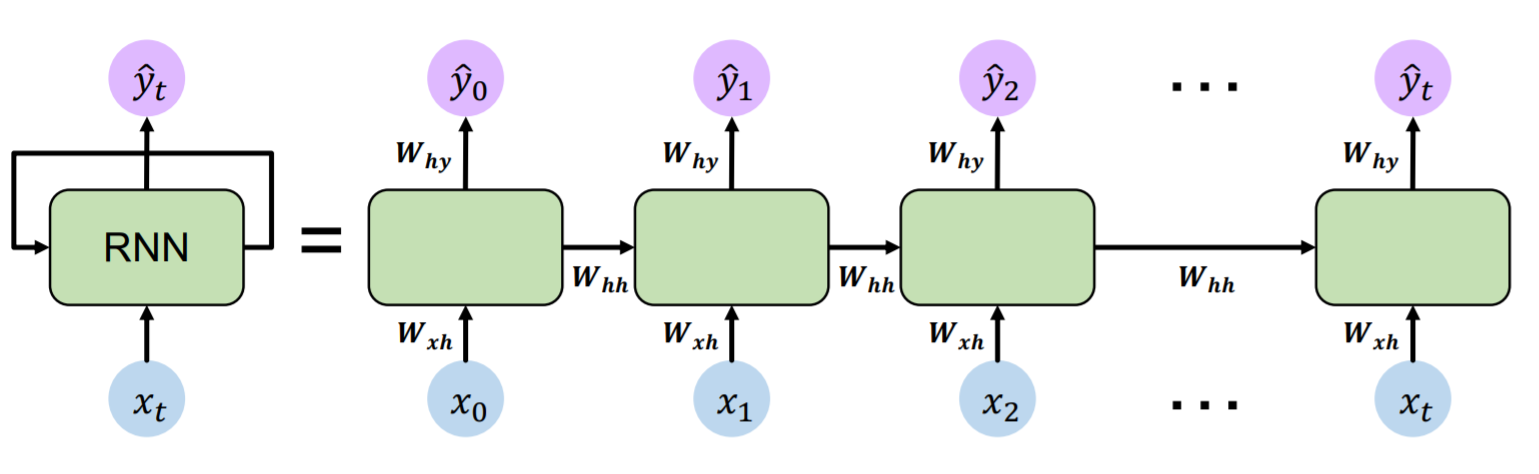
\includegraphics[height=3.5cm]{rnn}
    \caption{An unfolded RNN where $W_{hy}$ is the weight vector between the state and the output 
    , $W_{xh}$ is the weight vector between the current input $x_{t}$ and the state $h_{t}$ \cite{mitlectwo}.}
\end{figure}

\gls{rnns} proved to be useful in many applications. For example, 
text prediction \cite{jagannatha2016structured}, Self-Driving Cars \cite{gu2020lstm}, and climate analysis and prediction \cite{earthnet}.


\section{Conclusion}

In conclusion, \gls{anns} have many applications and usages that 
could change our society.
Unfortunately, we could not cover all of the architectures and applications of \gls{anns},
since there are many of them. To name a few, \gls{vae} which is used to generate data and 
reconstruct images \cite{hou2017deep} \cite{yan2016attribute2image}, and 
\gls{drl} which is seen in many applications, such as playing competitive computer games \cite{berner2019dota} and solving the Rubik cube \cite{openairubikcube}.
















% \begin{figure}
% 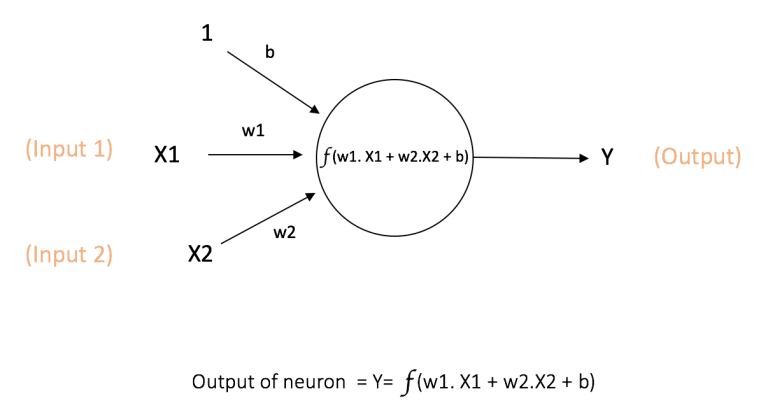
\includegraphics[height=6cm]{neuron}
% \caption{https://ujjwalkarn.me/2016/08/09/quick-intro-neural-networks/}
% \end{figure}


%
% ---- Bibliography ----
%
% BibTeX users should specify bibliography style 'splncs04'.
% References will then be sorted and formatted in the correct style.
%
\Urlmuskip=0mu plus 1mu\relax
\bibliographystyle{splncs04}
\bibliography{refs}
%
% \begin{thebibliography}{8}
% \bibitem{ref_article1}
% Author, F.: Article title. Journal \textbf{2}(5), 99--110 (2016)


% \bibitem{ref_lncs1}
% Author, F., Author, S.: Title of a proceedings paper. In: Editor,
% F., Editor, S. (eds.) CONFERENCE 2016, LNCS, vol. 9999, pp. 1--13.
% Springer, Heidelberg (2016). \doi{10.10007/1234567890}

% \bibitem{ref_book1}
% Author, F., Author, S., Author, T.: Book title. 2nd edn. Publisher,
% Location (1999)

% \bibitem{ref_proc1}
% Author, A.-B.: Contribution title. In: 9th International Proceedings
% on Proceedings, pp. 1--2. Publisher, Location (2010)

% \bibitem{ref_url1}
% LNCS Homepage, \url{http://www.springer.com/lncs}. Last accessed 4
% Oct 2017
% \end{thebibliography}
\end{document}
